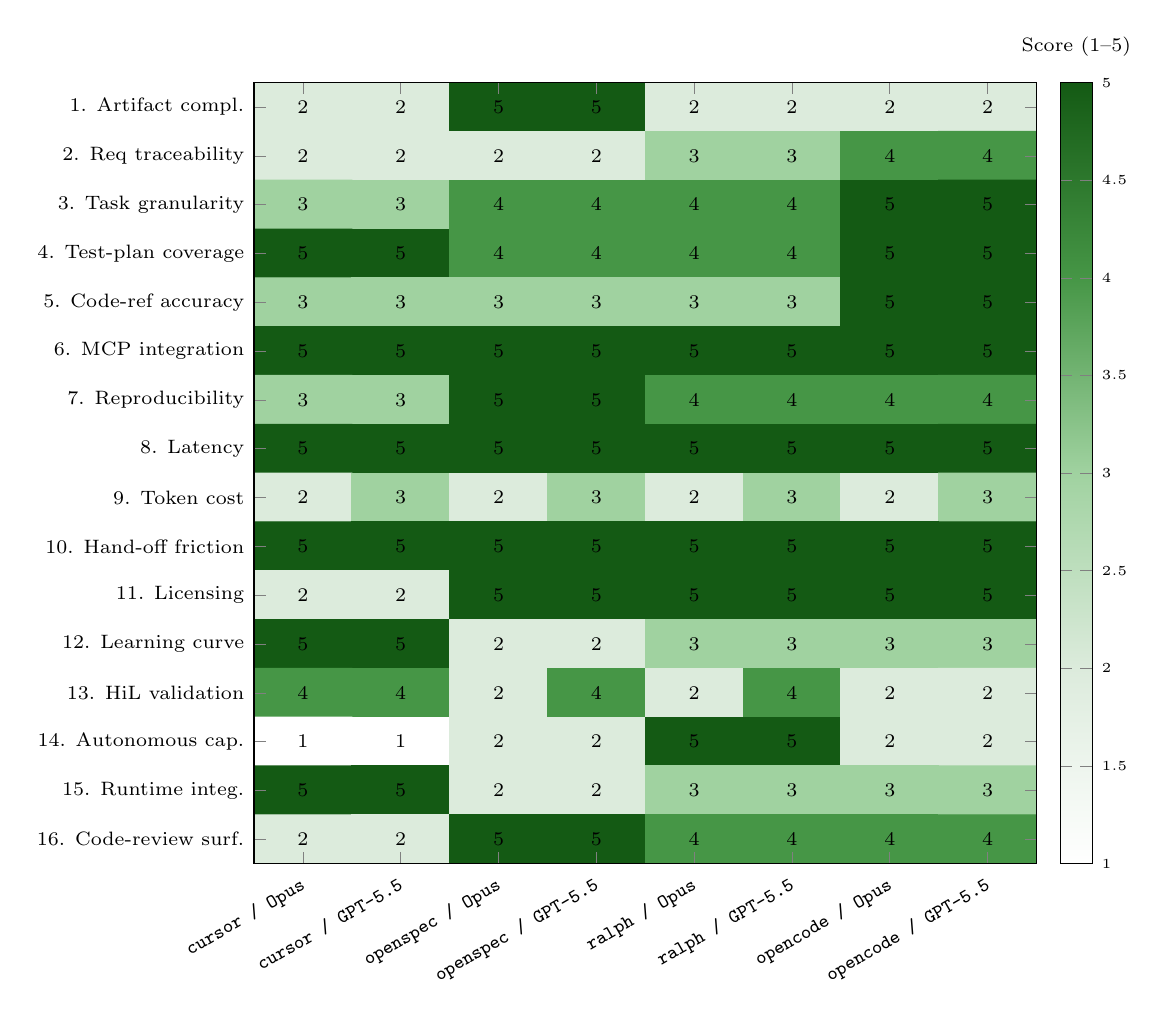
\begin{tikzpicture}[font=\scriptsize]
\begin{axis}[
  width=0.95\linewidth,
  height=11.5cm,
  view={0}{90},
  colormap={whgrn}{rgb255=(255,255,255) rgb255=(220,235,220) rgb255=(160,210,160) rgb255=(70,150,70) rgb255=(20,90,20)},
  point meta min=1, point meta max=5,
  xtick={0,1,2,3,4,5,6,7},
  xticklabels={
    {cursor / Opus},
    {cursor / GPT-5.5},
    {openspec / Opus},
    {openspec / GPT-5.5},
    {ralph / Opus},
    {ralph / GPT-5.5},
    {opencode / Opus},
    {opencode / GPT-5.5}
  },
  xticklabel style={rotate=30, anchor=north east, font=\scriptsize\ttfamily},
  ytick={0,1,2,3,4,5,6,7,8,9,10,11,12,13,14,15},
  yticklabels={
    {1. Artifact compl.},
    {2. Req traceability},
    {3. Task granularity},
    {4. Test-plan coverage},
    {5. Code-ref accuracy},
    {6. MCP integration},
    {7. Reproducibility},
    {8. Latency},
    {9. Token cost},
    {10. Hand-off friction},
    {11. Licensing},
    {12. Learning curve},
    {13. HiL validation},
    {14. Autonomous cap.},
    {15. Runtime integ.},
    {16. Code-review surf.}
  },
  yticklabel style={font=\scriptsize},
  enlargelimits=false,
  axis on top,
  colorbar,
  colorbar style={
    width=4mm,
    title={Score (1--5)},
    title style={font=\scriptsize},
    tick label style={font=\tiny},
  },
  nodes near coords*={\pgfmathprintnumber{\pgfplotspointmeta}},
  nodes near coords style={
    font=\scriptsize\bfseries,
    color=black,
    anchor=center,
    inner sep=0pt,
  },
]
\addplot[matrix plot,
         mesh/cols=8,
         point meta=explicit] table[meta=score] {
x  y  score
0  0  2
1  0  2
2  0  5
3  0  5
4  0  2
5  0  2
6  0  2
7  0  2
0  1  2
1  1  2
2  1  2
3  1  2
4  1  3
5  1  3
6  1  4
7  1  4
0  2  3
1  2  3
2  2  4
3  2  4
4  2  4
5  2  4
6  2  5
7  2  5
0  3  5
1  3  5
2  3  4
3  3  4
4  3  4
5  3  4
6  3  5
7  3  5
0  4  3
1  4  3
2  4  3
3  4  3
4  4  3
5  4  3
6  4  5
7  4  5
0  5  5
1  5  5
2  5  5
3  5  5
4  5  5
5  5  5
6  5  5
7  5  5
0  6  3
1  6  3
2  6  5
3  6  5
4  6  4
5  6  4
6  6  4
7  6  4
0  7  5
1  7  5
2  7  5
3  7  5
4  7  5
5  7  5
6  7  5
7  7  5
0  8  2
1  8  3
2  8  2
3  8  3
4  8  2
5  8  3
6  8  2
7  8  3
0  9  5
1  9  5
2  9  5
3  9  5
4  9  5
5  9  5
6  9  5
7  9  5
0  10 2
1  10 2
2  10 5
3  10 5
4  10 5
5  10 5
6  10 5
7  10 5
0  11 5
1  11 5
2  11 2
3  11 2
4  11 3
5  11 3
6  11 3
7  11 3
0  12 4
1  12 4
2  12 2
3  12 4
4  12 2
5  12 4
6  12 2
7  12 2
0  13 1
1  13 1
2  13 2
3  13 2
4  13 5
5  13 5
6  13 2
7  13 2
0  14 5
1  14 5
2  14 2
3  14 2
4  14 3
5  14 3
6  14 3
7  14 3
0  15 2
1  15 2
2  15 5
3  15 5
4  15 4
5  15 4
6  15 4
7  15 4
};
\end{axis}
\end{tikzpicture}
